
To start the development of our GUI prototypes,  GUI wire frames were drafted for the main order/service screen, the main inventory screen, add stock and item screens. \\

Figure \ref{fig:Service_window_A} below shows a first draft of the order/service window. The main idea behind this design was to have large buttons for each item and a tabbed menu selector along the top for selecting categories. It also includes the idea of having an edit button for each item in the order.

\begin{figure}[ht]
	\centering
	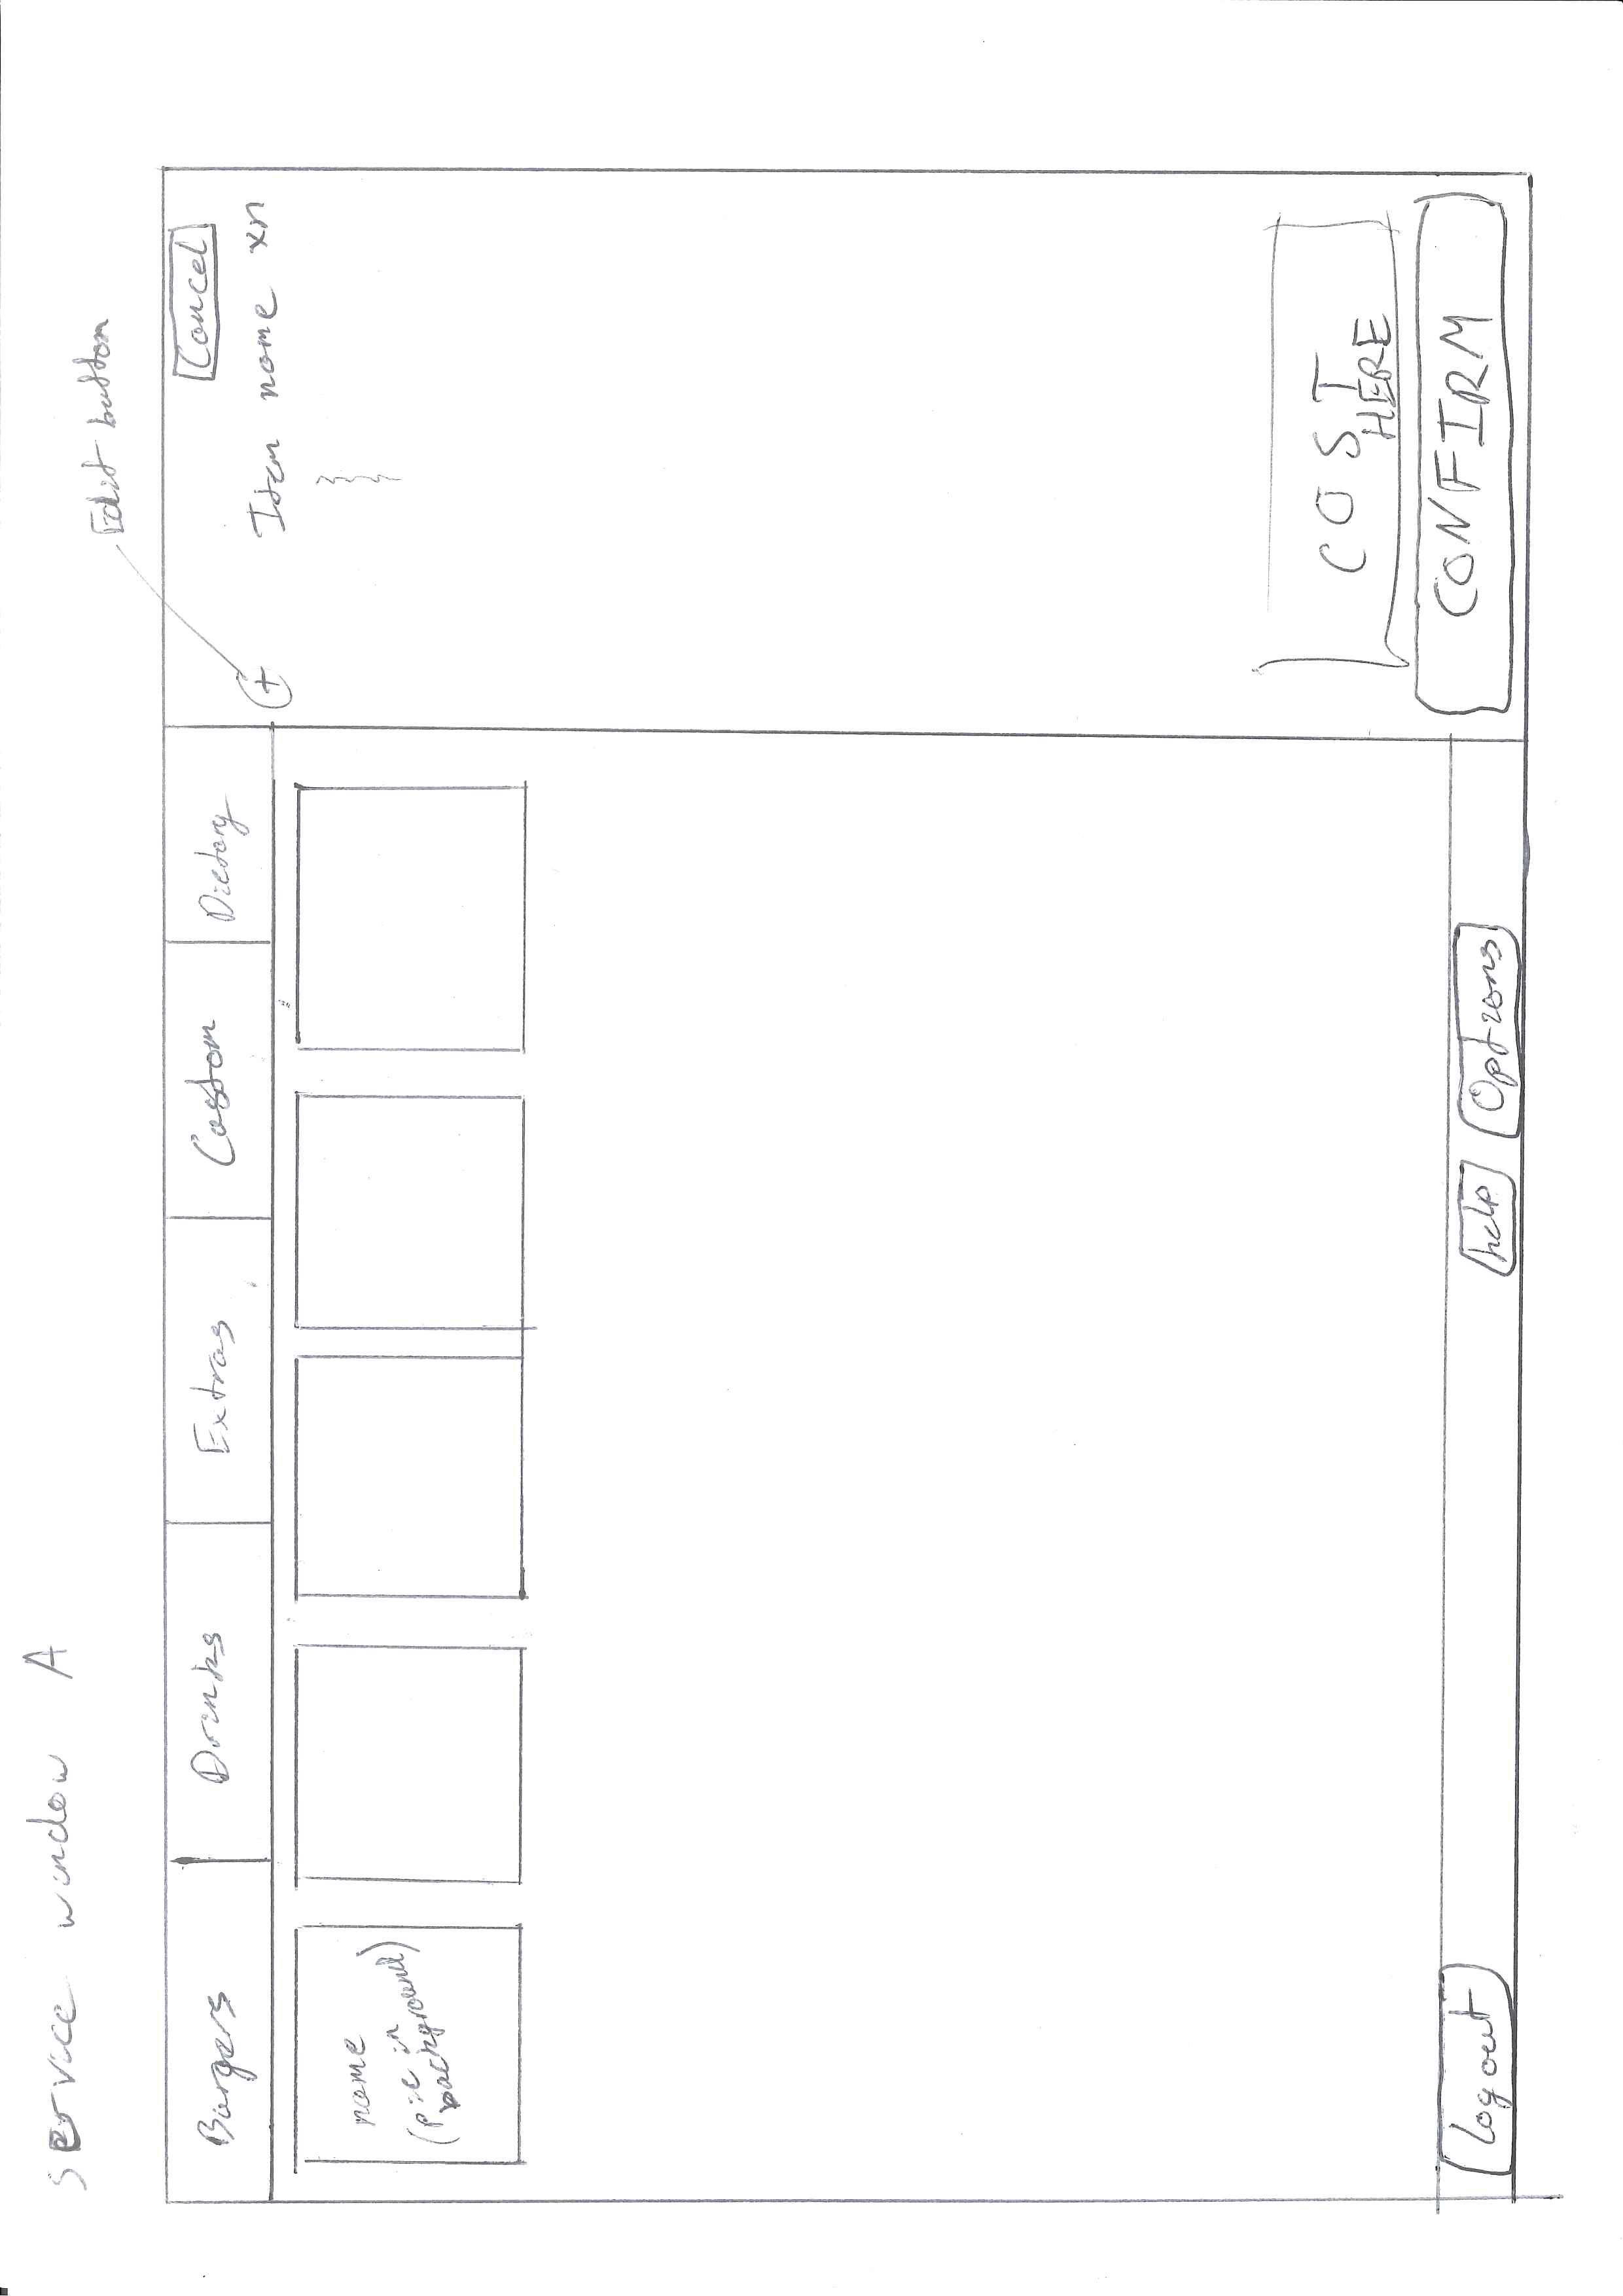
\includegraphics[width=100mm,angle=-90]{images/Wireframe_drafts/Service_window_A.jpg}
	\caption{Initial wire frame design of the order screen}
	\label{fig:Service_window_A}
\end{figure}

After the initial wire frames it was realised that going out and surveying relevant stakeholders to find out what is important in a POS system would allow us to ensure that further development worked towards bettering the design. To such ends we talked to the Reboot café and the doughnut food truck on campus. The full questions and answers can be found in Section \ref{subsec:StakeholderSurvey}.

After this feedback from some end users more in depth GUI prototypes were developed using the online tool moqups. During this time we also took inspiration from the Reboot café and decided to colour code each of the item buttons to help with usability.
\pagebreak

\begin{figure}[ht]
	\centering
	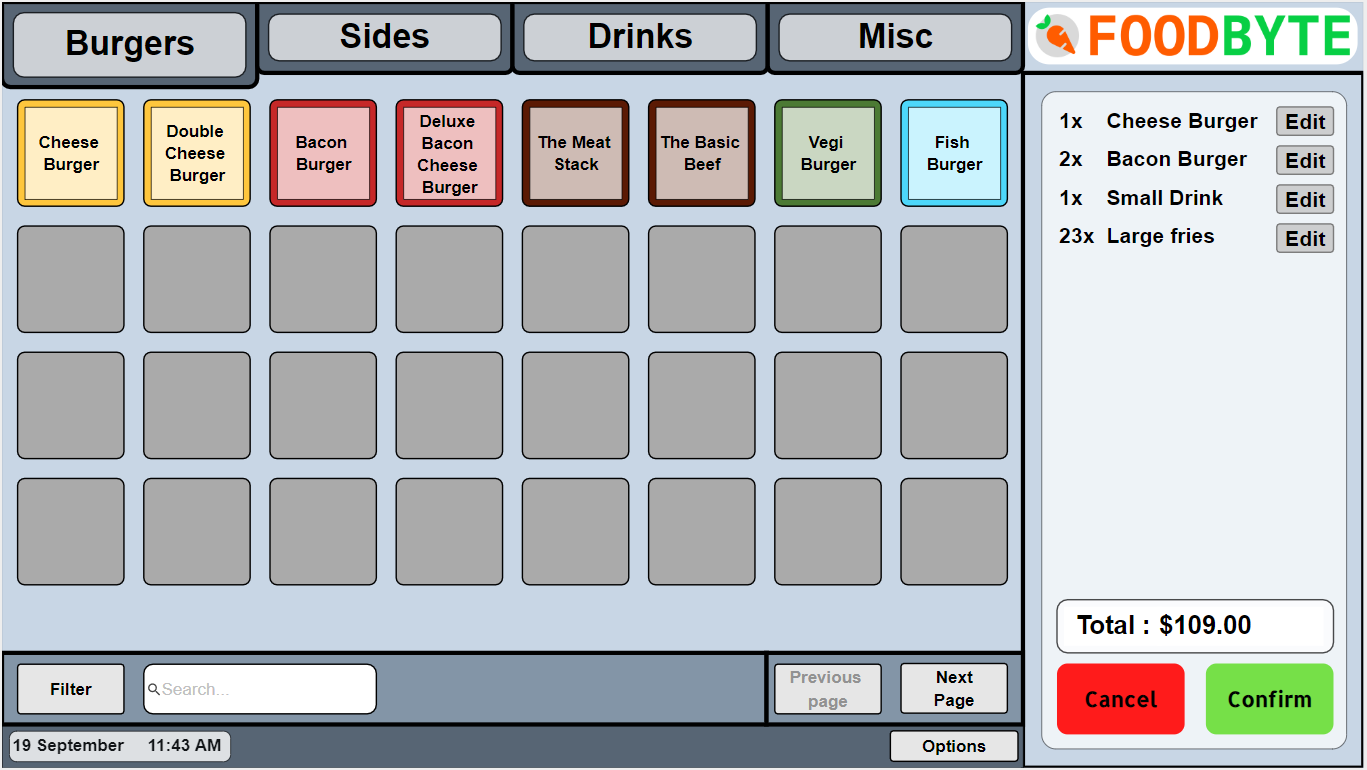
\includegraphics[width=150mm]{images/GUI_prototypes/Order_screen.PNG}
	\caption{Refined mock up of the order screen}
	\label{fig:order_screen_moqueup}
\end{figure}

In this GUI prototype (see Figure \ref{fig:order_screen_moqueup}) several of the features, quality requirements and their use cases have been taken into consideration. Each item has a large button that is colour coded based on what it is (ie. cheese based/featuring items are yellow). This helps with the usability of the GUI (QR3) as well as directly implementing the ability to add an item to the current order (FR4). There is a clear and large cancel button to allow for the cancelling of orders (FR6). The running total cost of the order is clearly displayed above the order confirmation button (FR3). The order confirmation button opens a popup for the order confirmation where, if payment is via cash, the change can be calculated (FR2). Each item in the current order has an edit button to allow for items to be edited (FR8, FR9). It can also be noted that there are selectable tabs for different categories as well as options to search and/or filter items. The date and time is displayed in the bottom left as this is a convenient feature to have during service. The next/previous page buttons are to allow for an overflow of items as page switching can be more reliable than scrolling (QR2). Finally there is an “Options” button that opens a pop-up with access to the management side of the application as well as the ability to modify aspects of the service side (ie. prices). The options pop-up also has a button to bring up an order history to facilitate providing refunds (FR7).
The prototype sub windows and pop-ups related to the order screen can be found in the appendices.

\begin{figure}[ht]
	\centering
	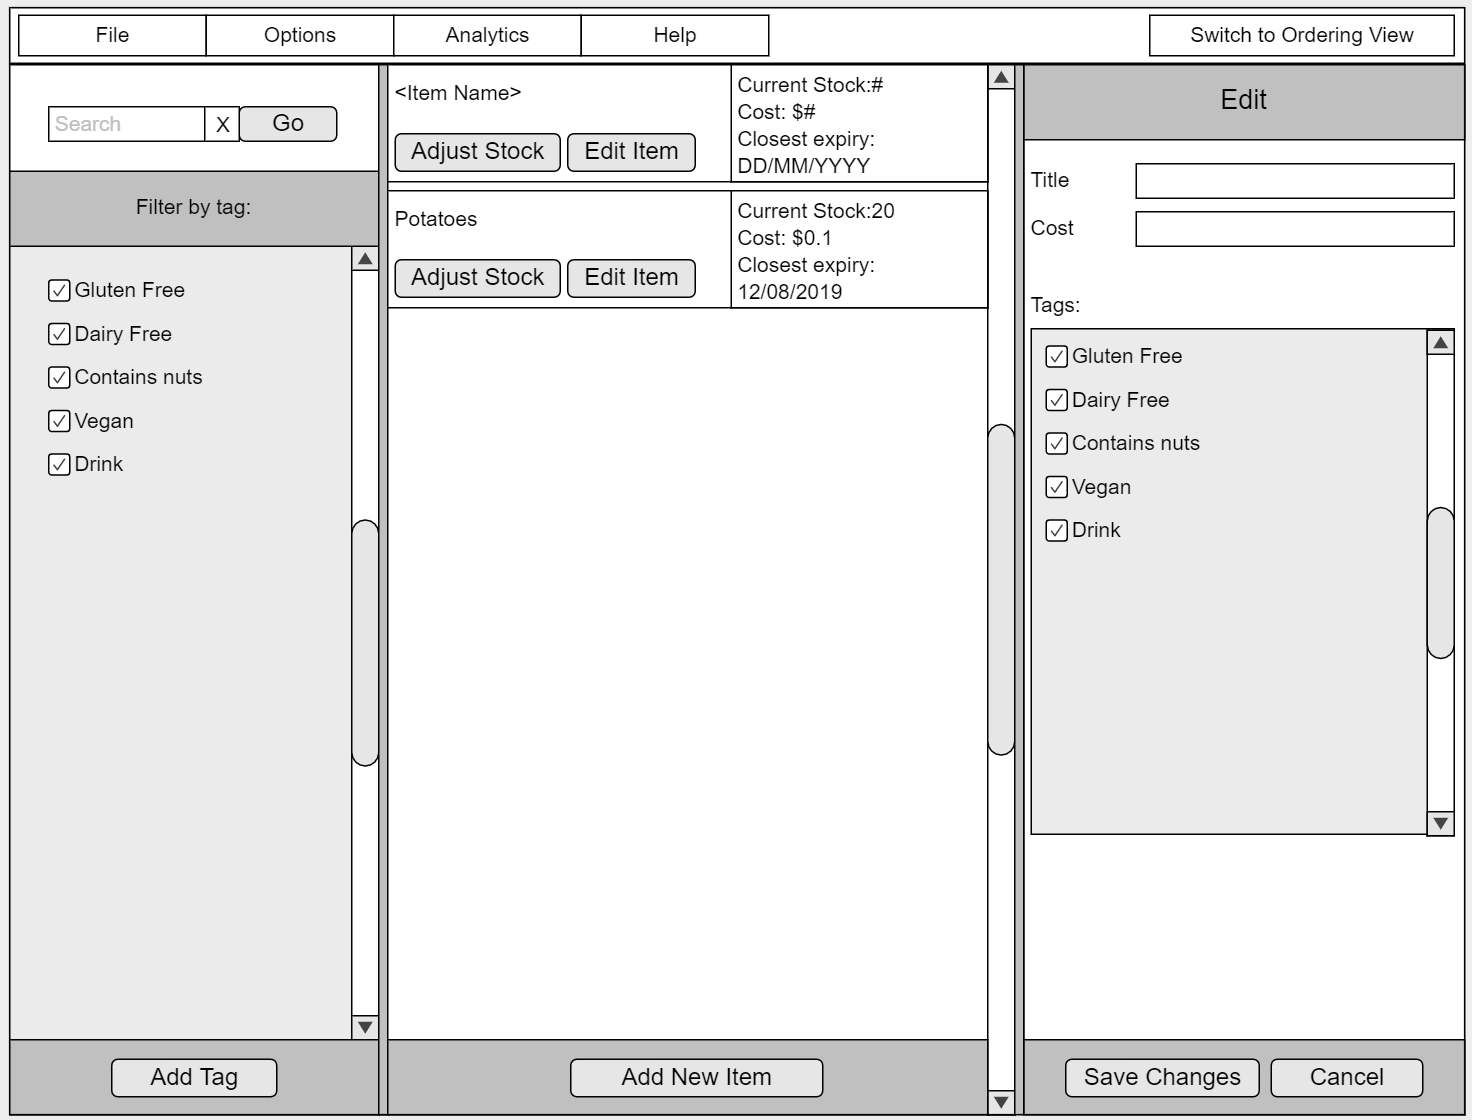
\includegraphics[width=150mm]{images/GUI_prototypes/Inventory_screen.png}
	\caption{Refined mock up of the inventory management screen}
	\label{fig:management_screen_moqueup}
\end{figure}

Figure \ref{fig:management_screen_moqueup}) shows a prototype design for the Inventory management system that features tools for stock management and product management. On the left there are options for filtering and searching items which will appear in the middle (FR16, FR19). Items can be added with the “Add New Item” button in the middle (FR20, FR18, FR10). Each item will have the current quantity displayed as well as the cost of the item and nearest expiry date, this will be alongside buttons to adjust stock level and edit item (FR20, FR14, FR24). On the right is the edit screen for editing a selected item, this could also be used for creating new items (FR13, FR10). At the top there are buttons for file which would allow for import/export (FR25, FR26) as well as a button to switch back to operational view (FR21).